% Auto-generated by experiments/build_embedding_clusters.py
\begin{figure}[!htb]
\centering
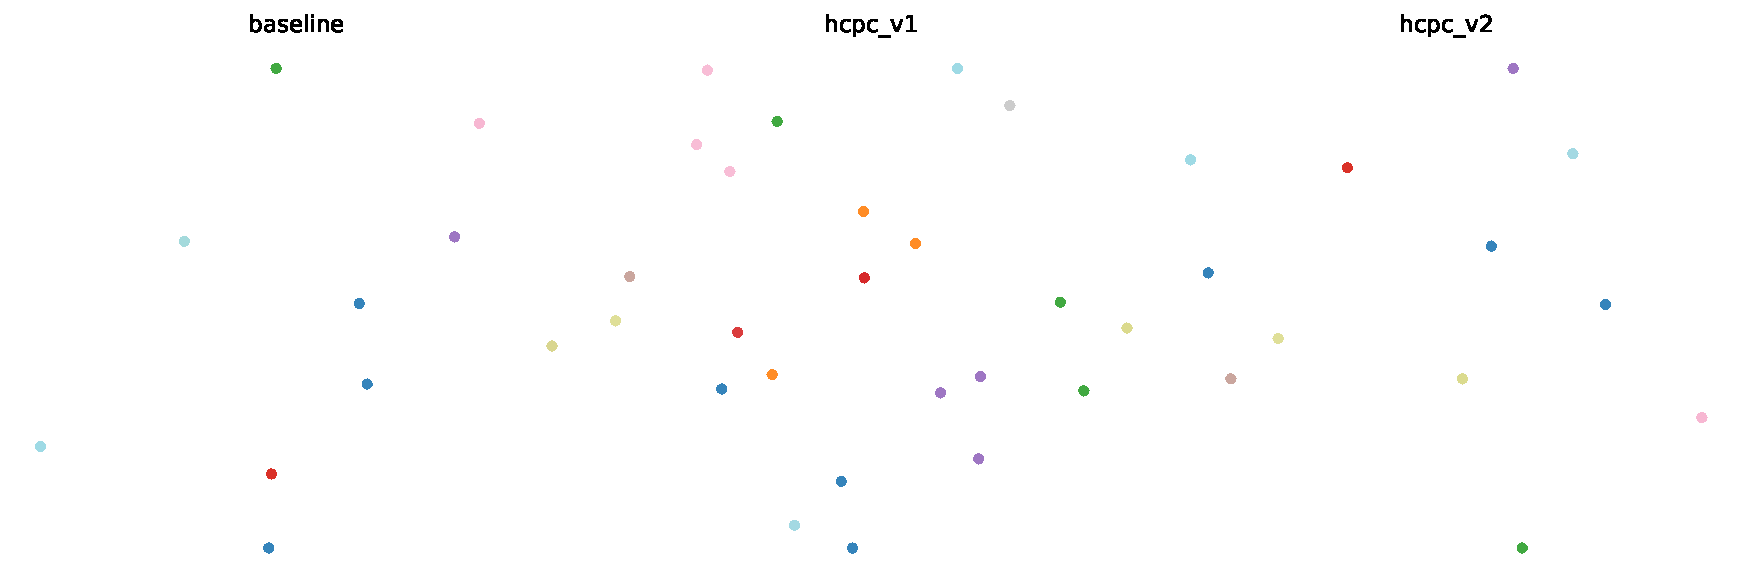
\includegraphics[width=\linewidth]{figures/embedding_clusters.pdf}
\caption{\textbf{Embedding-space view of the refinement paradox.}
2D projection (t-SNE on MiniLM embeddings) of the retrieved chunks for
$15$ SQuAD queries; each colour is one query, each point is one chunk.
\textbf{Left (baseline):} per-query chunks form tight same-colour
clusters --- evidence is locally consistent within each query.
\textbf{Centre (HCPC-v1):} the same colours scatter across the plot ---
per-passage refinement has substituted in chunks from elsewhere in the
corpus that match each individual question independently but no longer
form a coherent set.
\textbf{Right (HCPC-v2):} per-query clusters return, because the
selective refinement policy declines to refine when doing so would
shatter the original cluster.}
\label{fig:embedding_clusters}
\end{figure}
